\subsection{Hàm}
\subsubsection{Hàm 1}
\textbf{Mô tả hàm 1:} Hàm tinhluong có chức năng tính lương trước thuế cho một nhân viên nhất định, với thời gian tính lương được xác định bởi người dùng

\textbf{Input:} 
\begin{itemize}
    \item [--] Tham số MaNV, có kiểu \texttt{CHAR(6)} 
    \item [--] Tham số ngayBatDau, có kiểu \texttt{DATE} 
    \item [--] Tham số ngayKetThuc, có kiểu \texttt{DATE} 
\end{itemize}

\textbf{Output:} Giá trị luong, có kiểu \texttt{INT}, mang ý nghĩa là lương trước thuế của nhân viên trong khoảng thời gian cho trước.

\textbf{Câu lệnh khởi tạo hàm}
\begin{minted}{mysql}
CREATE FUNCTION tinhLuong (MaNV CHAR(6), ngayBatDau DATE, ngayKetThuc DATE) RETURNS INT DETERMINISTIC
BEGIN
    DECLARE luong INT DEFAULT 0;
    DECLARE current_workingDate DATE;
    DECLARE current_luong INT;
    DECLARE done INT DEFAULT 0;

    -- Declare a cursor to iterate through workdays and daily salaries
    DECLARE WorkDay_CURSOR CURSOR FOR
        SELECT `Ngay`, `TongSoGioLam`*`LuongTheoGio`
        FROM bangchamcong NATURAL INNER JOIN nhanvien
        WHERE nhanvien.MaNV = MaNV;

    -- Declare a handler for the end of the cursor
    DECLARE CONTINUE HANDLER FOR NOT FOUND SET done = 1;
\end{minted}
\begin{minted}[firstnumber=16]{mysql}
    -- Input validation: Check if MaNV exists
    IF MaNV IS NULL OR NOT EXISTS (
    SELECT 1 
    FROM nhanvien 
    WHERE nhanvien.`MaNV` = MaNV
    ) THEN
    RETURN -1; -- Invalid employee ID
    END IF;

    -- Validate the date range
    IF ngayBatDau IS NULL OR ngayKetThuc IS NULL OR ngayBatDau > ngayKetThuc THEN
    RETURN -2; -- Invalid date range
    END IF;

    -- Open the cursor
    OPEN WorkDay_CURSOR;

    -- Loop through the cursor
    read_loop: LOOP
        FETCH WorkDay_CURSOR INTO current_workingDate, current_luong;
        IF done = 1 THEN
            LEAVE read_loop;
        END IF;

        -- Check if the working date is within the specified range
        IF (current_luong is NOT NULL) AND (current_workingDate BETWEEN ngayBatDau AND ngayKetThuc) THEN
            SET luong = luong + current_luong;
        END IF;
    END LOOP;

    -- Close the cursor
    CLOSE WorkDay_CURSOR;

    RETURN luong;
END //
\end{minted}

\newpage
\textbf{Kiểm tra}: Tính lương của nhân viên có mã nhân viên là "NV7733" từ ngày 01/11/2024 đến 07/11/2024:
\begin{itemize}
    \item [--] Thông tin về nhân viên và giờ làm việc của nhân viên trên từ ngày 01/11/2024 đến 07/11/2024:
    \begin{figure}[H]
        \centering
        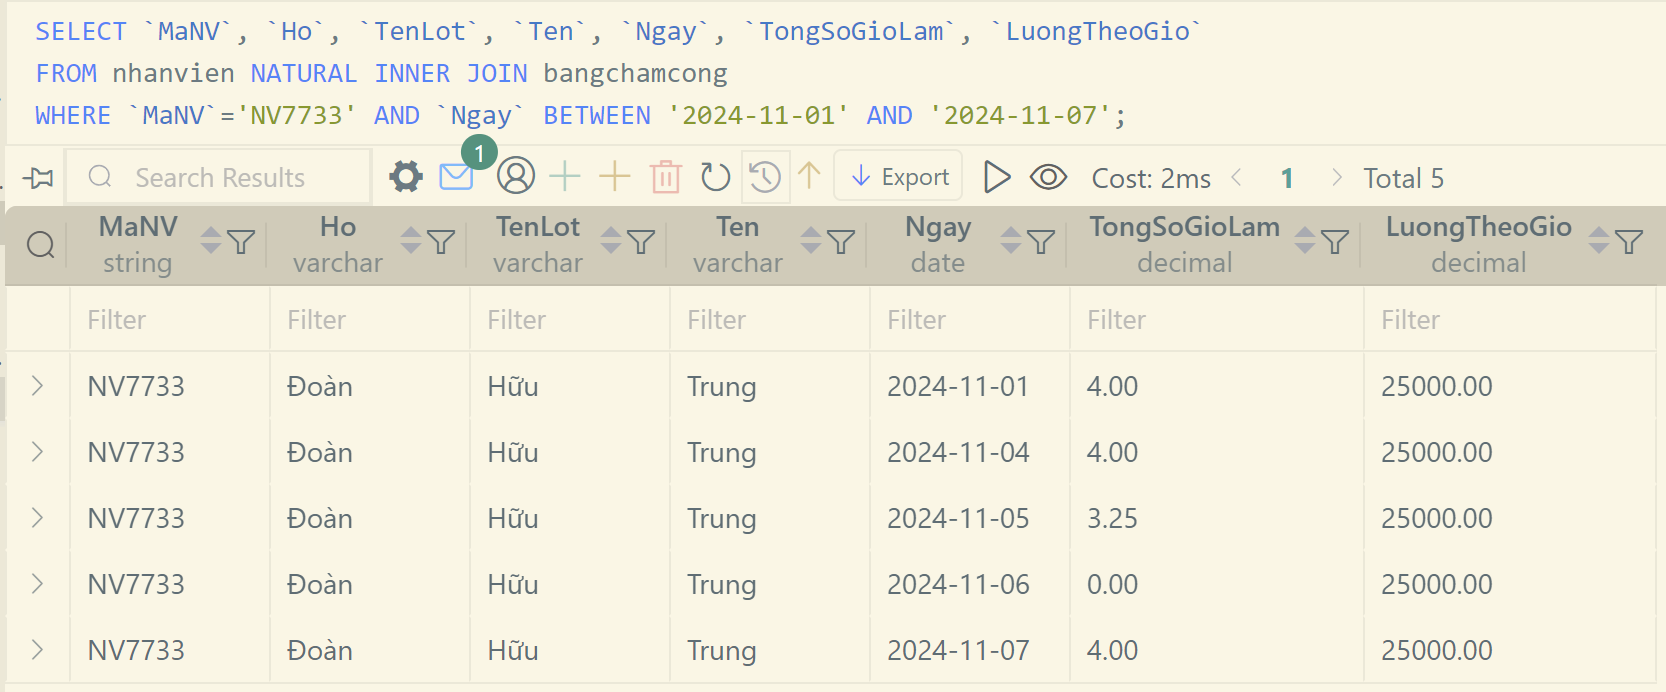
\includegraphics[width=\linewidth]{content/images/func_1_1.png}
        \caption{Thông tin về nhân viên và giờ làm việc của nhân viên}
        \label{fig:func_1_1}
    \end{figure}
    \item [--] Có thể thấy, lương của nhân viên 'NV7733' trong quãng thời gian trên là:
    $$
    (4.00 + 4.00 + 3.25 + 0.00 + 4.00) \times 25000 = 381250
    $$
    \item [--] Giá trị mà hàm trả về đúng bằng giá trị vừa tính được:
    \begin{figure}[H]
        \centering
        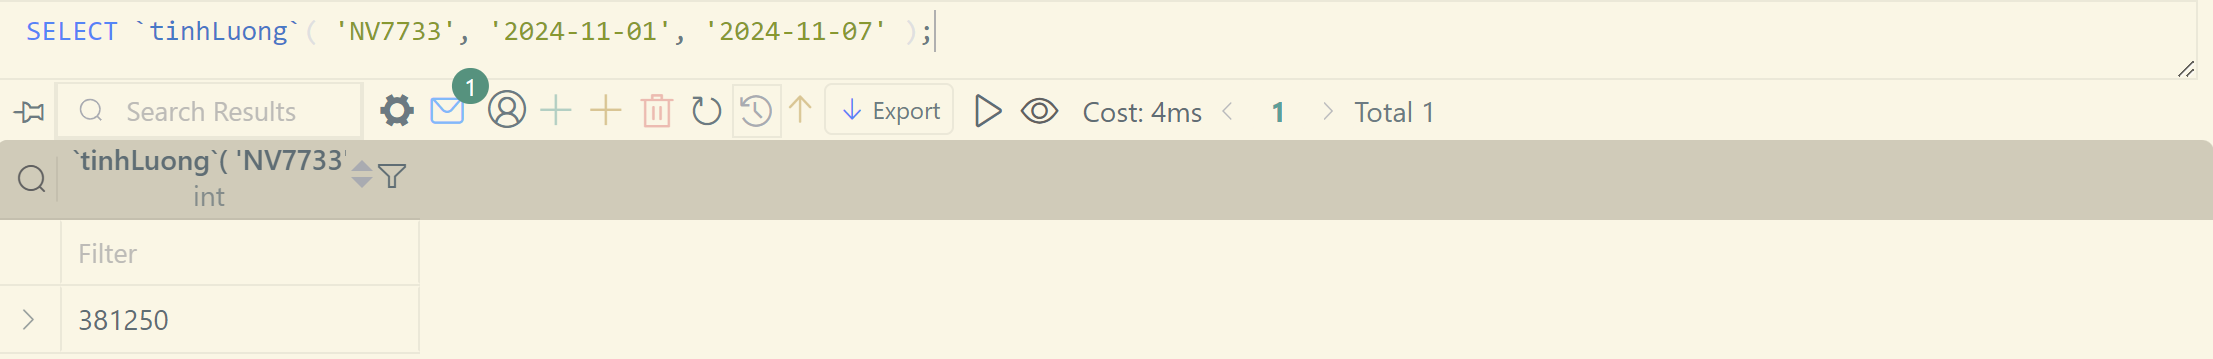
\includegraphics[width=\linewidth]{content/images/func_1_2.png}
        \caption{Kết quả sau khi gọi hàm tinhluong}
        \label{fig:func_1_2}
    \end{figure}
\end{itemize}

\newpage
\subsubsection{Hàm 2}
\textbf{Mô tả hàm 2:} Hàm KiemTraTangCa có chức năng kiểm tra số giờ tăng ca của một nhân viên có vượt quá số giờ được truyền vào không trong một quãng thời gian được người gọi hàm quy định.

\textbf{Input:} 
\begin{itemize}
    \item [--] Tham số MaNV, có kiểu \texttt{CHAR(6)} 
    \item [--] Tham số NgayBatDau, có kiểu \texttt{DATE} 
    \item [--] Tham số NgayKetThuc, có kiểu \texttt{DATE} 
    \item [--] Tham số GioTangCaToiThieu, có kiểu \texttt{TIME} 
\end{itemize}

\textbf{Output:} Giá trị BOOLEAN, trả về 0 nếu thời gian tăng ca là nhỏ hơn, ngược lại trả về 1.

\textbf{Câu lệnh khởi tạo hàm}
\begin{minted}{mysql}
CREATE Function KiemTraTangCa (MaNV CHAR(6), NgayBatDau Date, NgayKetThuc Date, GioTangCaToiThieu TIME) RETURNS BOOLEAN DETERMINISTIC
BEGIN 
    DECLARE total_hours TIME DEFAULT 0;
    DECLARE current_gioTangCa TIME;
    DECLARE current_ngay DATE;
    DECLARE done INT DEFAULT 0;
    -- DECLARE 
    DECLARE nhungLanRaVao CURSOR FOR 
        SELECT TIMEDIFF(lanravao.`GioRa`, lanravao.`GioVao`), lanravao.`Ngay`
        FROM lanravao 
        WHERE `GioVao` > '17:00:00' AND lanravao.`MaNV` = `MaNV`;

    DECLARE CONTINUE HANDLER FOR NOT FOUND SET done = 1;
    
    IF MaNV is NULL OR NOT EXISTS (SELECT 1 FROM nhanvientoanthoigian WHERE nhanvientoanthoigian.`MaNV` = `MaNV`) THEN 
        RETURN -1; -- MaNV rỗng hoặc MaNV không phải là NV toàn thời gian;
    END IF; 

\end{minted}
\begin{minted}[firstnumber=19]{mysql}
    IF NgayBatDau IS NULL OR NgayKetThuc IS NULL OR (NgayKetThuc < NgayBatDau) THEN 
        RETURN -2; -- NgayBatDau hoặc NgayKetThuc rỗng hoặc phạm vi ngày không hợp lệ
    END IF;

    IF GioTangCaToiThieu IS NULL THEN
        RETURN -3; -- GioTangCaToiThieu rỗng
    END IF;

    OPEN nhungLanRaVao;
    read_loop: LOOP
    FETCH nhungLanRaVao into current_gioTangCa, current_ngay;
    IF done = 1 THEN
        LEAVE read_loop;
    END IF;

    IF current_ngay BETWEEN NgayBatDau AND NgayKetThuc THEN
        SET total_hours = ADDTIME(total_hours, current_gioTangCa);
    END IF;
END LOOP;

CLOSE nhungLanRaVao;

return (total_hours >= GioTangCaToiThieu);
END //
\end{minted}
\newpage
\textbf{Kiểm tra}: Kiểm tra tổng số giờ tăng ca của nhân viên có mã nhân viên là 'NV1271' xem trong thời gian từ ngày 01/11/2024 đến ngày 30/11/2024, thời gian tăng ca của nhân viên đó có vượt qua mốc 7 tiếng và 8 tiếng không.
\begin{itemize}
    \item [--] Truy vấn tổng thời gian tăng ca bằng câu lệnh SELECT, có thể thấy tổng giờ tăng ca từ ngày 01/11/2024 đến ngày 30/11/2024 của nhân viên 'NV1271' là 7 tiếng 11 phút.
    \begin{figure}[H]
        \centering
        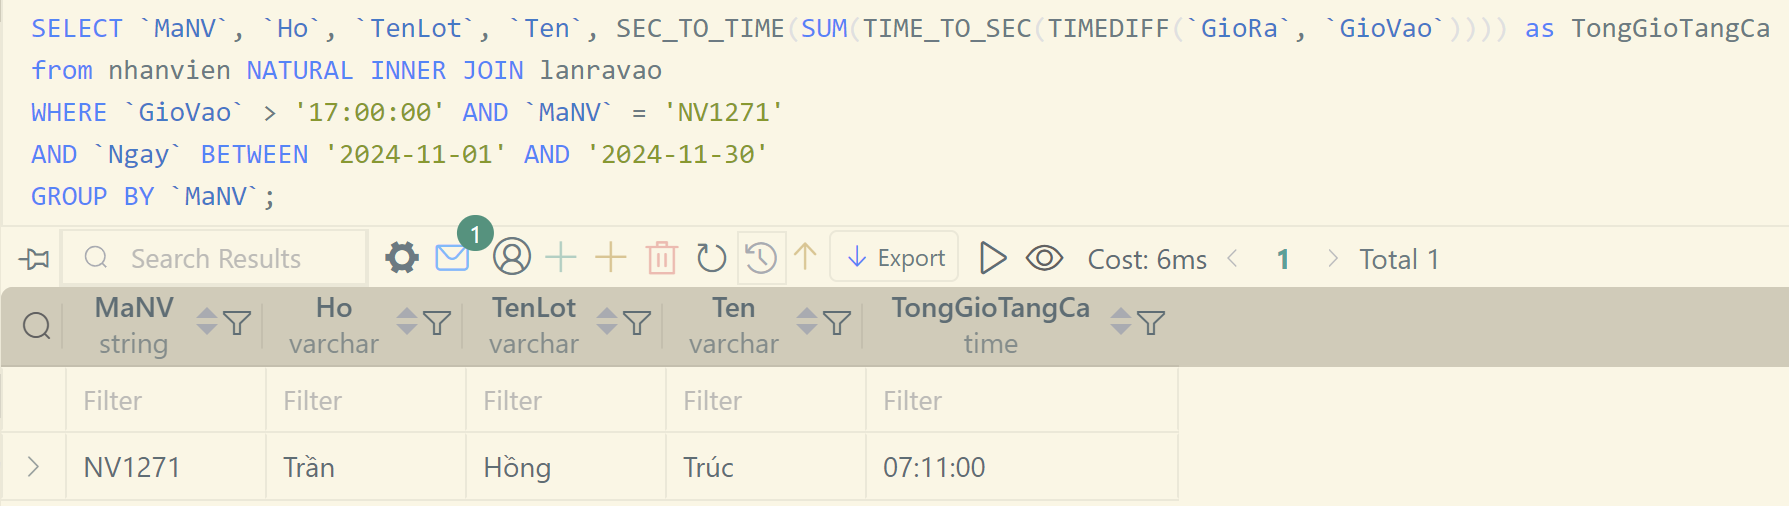
\includegraphics[width=\linewidth]{content/images/func_2_1.png}
        \caption{Kết quả truy vấn}
        \label{fig:func_2_1}
    \end{figure}
    \item [--] Gọi hàm để kiểm tra với số giờ là 7 tiếng, kết quả cho ra là 1 (True), đúng với kỳ vọng
    \begin{figure}[H]
        \centering
        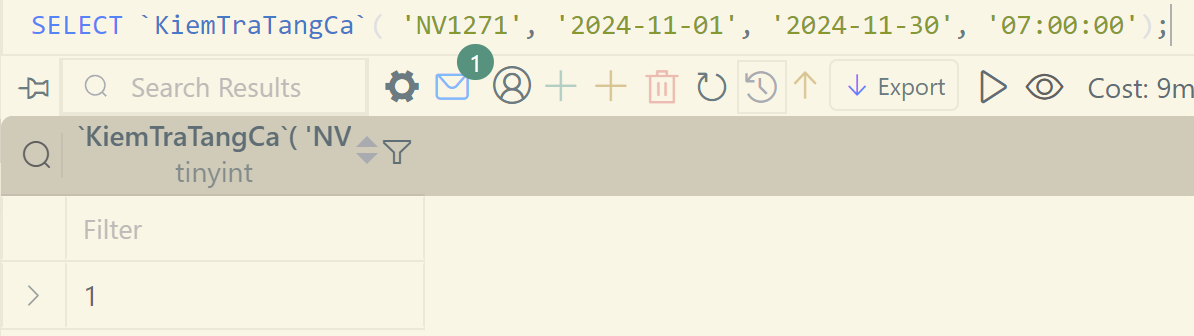
\includegraphics[width=\linewidth]{content/images/func_2_2.png}
        \caption{Kết quả sau khi gọi hàm KiemTraTangCa}
        \label{fig:func_2_2}
    \end{figure}
    \item [--] Gọi hàm để kiểm tra với số giờ là 8 tiếng, kết quả cho ra là 0 (False), đúng với kỳ vọng
    \begin{figure}[H]
        \centering
        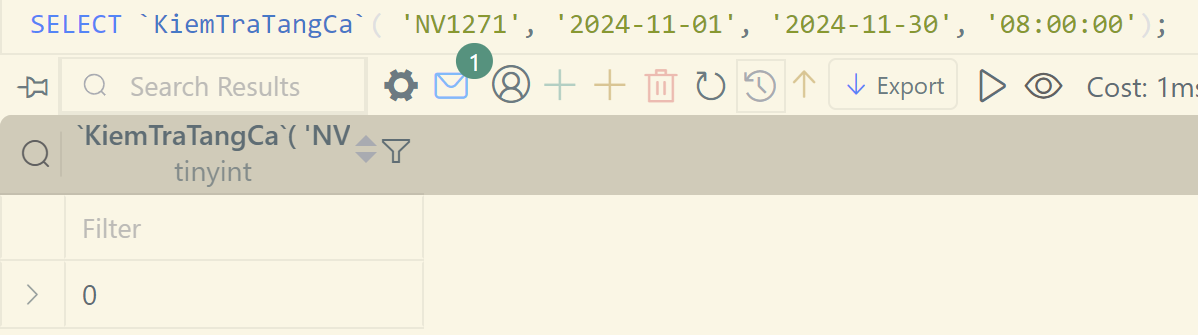
\includegraphics[width=\linewidth]{content/images/func_2_3.png}
        \caption{Kết quả sau khi gọi hàm KiemTraTangCa}
        \label{fig:func_2_3}
    \end{figure}
\end{itemize}
\newpage